% Chapter Template

\chapter{Elderly care demo} % Main chapter title

\label{Chapter7} % Change X to a consecutive number; for referencing this chapter elsewhere, use \ref{ChapterX}

%----------------------------------------------------------------------------------------
%	SECTION 1
%----------------------------------------------------------------------------------------
The chapter will first address the issue being solved,
then the methodology will be presented, and finally,
the results will be disclosed.

Elderly care has been addressed by many EU-funded research projects since the aging population is one of the main issues the union is facing. 

There are many solutions to this problem.
One approach is invasive such as wearables, sound sensors, IR occupancy detectors, etc. 
Few authors tried to solve this issue using non-invasive using previously mentioned NILM algorithms. 
In this case, no additional meters need to be installed, since per-appliance usage can be disaggregated.
While this is practical from the new equipment side, it is a bit less practical from the efficiency and accuracy side, especially for larger buildings. 

There is a middle way between invasive and non-invasive approaches. 
It is possible to use sub-meters for each appliance and indirectly observe the usage pattern. 
The upside of this approach is that the elder does not need to wear the device.
The downside is, that this approach will be slower at detecting the accident.

\section{Goal}

The chapter will focus on building the elderly care system that will use users' periodic usage patterns to detect an anomaly.
The anomaly could be anything from a fall, stroke or altered usage pattern due to dementia. 
The algorithm will be designed based on the load profile from the previous chapter \ref{fig:PHPA}.
Figure shows, that first thing in the morning used are kettle and toaster, and with a delay of one hour, microwave and TV. 
If none of these appliances are used within that hour, then that hour is considered anomalous.
This means that the algorithm will be able to detect the anomaly within 1 hour of the accident.

\section{Methodology}

\subsection{Building anomaly detection algorithm}

The next section will present the steps taken while designing this algorithm.

\subsubsection{Step one}
To detect the anomalies one first needs to build a daily activation profile for each appliance, such as the one previously mentioned \ref{fig:PHPA}.
In this specific case, we will be using 2h buckets, yielding a total of 12 buckets. 

\subsubsection{Step two}
The second step is to ignore appliances that are always on by calculating the standard deviation of activations for each bucket. 
The activations are normalized between 0 and 1. 
This step is important so that appliances that are always on, such as fridge or freezer get ignored. 
These appliances are detected based on the width of their activation normal distribution. 
Where periodic (hourly basis) appliances should have narrow distributions, the more dynamic should have wider distributions.
This can be seen in examples from building 2.

\begin{figure}[H]
    \centering
    \begin{tikzpicture}
        \coordinate (s) at (0,0);
        \foreach \num in {866, 842, 810, 772, 868, 854, 859, 854, 864, 887, 889, 883}{
        \node[minimum size=6mm, draw, rectangle] at (s) {\num};
        \coordinate (s) at ($(s) + (1,0)$);
        }
    \end{tikzpicture}
    \caption{Daily activations for fridge $\sigma$ = 0.036}
    \label{arr:fridge_acts}
\end{figure}

\begin{figure}[H]
    \centering
    \begin{tikzpicture}
        \coordinate (s) at (0,0);
        \foreach \num in {86, 77, 75, 74, 100, 118, 113, 127, 168, 202, 171, 121}{
        \node[minimum size=6mm, draw, rectangle] at (s) {\num};
        \coordinate (s) at ($(s) + (1,0)$);
        }
    \end{tikzpicture}
    \caption{Daily activations for audio system $\sigma$ = 0.2}
    \label{arr:as_acts}
\end{figure}

\begin{figure}[H]
    \centering
    \begin{tikzpicture}
        \coordinate (s) at (0,0);
        \foreach \num in {9, 4, 4, 3, 212, 122, 85, 80, 102, 260, 134, 48}{
        \node[minimum size=6mm, draw, rectangle] at (s) {\num};
        \coordinate (s) at ($(s) + (1,0)$);
        }
    \end{tikzpicture}
    \caption{Daily activations for microwave $\sigma$ = 0.3}
    \label{arr:microwave_acts}
\end{figure}

Based on results from all appliances a threshold of $\sigma$ = 0.1 was set.
This method will also get rid of appliances that are always on due to their specific nature such as server computers 
or are rarely used. 

\subsubsection{Third step}

Next, appliances that trigger together must be grouped. 
This means we must find part of the day that they are operating.
Due to the filter in the previous step, we are left with appliances whose usage variates trough the day. 
Some appliances are on even when the user is not necessarily using them, this can be seen in figure \ref{arr:as_acts}.
One out of many ways to do this is to normalize the activations, this yields a metric that tells us the probability of that appliance being turned on compared to the rest of the day. 
If we do this for same appliances as above the result is following: 

\begin{figure}[H]
    \centering
    \begin{tikzpicture}
        \coordinate (s) at (0,0);
        \foreach \num in {0.43, 0.38, 0.37, 0.37, 0.5 , 0.58, 0.56, 0.63, 0.83, 1. , 0.85,
        0.6}{
        \node[minimum size=6mm, draw, rectangle] at (s) {\num};
        \coordinate (s) at ($(s) + (1,0)$);
        }
    \end{tikzpicture}
    \caption{Daily activations for audio system $\sigma$ = 0.2}
    \label{arr:as_acts_norm}
\end{figure}

\begin{figure}[H]
    \centering
    \begin{tikzpicture}
        \coordinate (s) at (0,0);
        \foreach \num in {0.03, 0.02, 0.02, 0.01, 0.82, 0.47, 0.33, 0.31, 0.39, 1.  , 0.52,
        0.18}{
        \node[minimum size=6mm, draw, rectangle] at (s) {\num};
        \coordinate (s) at ($(s) + (1,0)$);
        }
    \end{tikzpicture}
    \caption{Daily activations for microwave $\sigma$ = 0.3}
    \label{arr:microwave_acts_norm}
\end{figure}

Finally, a suitable threshold must be selected.
The threshold of 0.5 was selected, which yields the following vectors:

\begin{figure}[H]
    \centering
    \begin{tikzpicture}
        \coordinate (s) at (0,0);
        \foreach \num in {0, 0, 0, 0, 0 , 1, 1, 1, 1, 1 , 1, 1}{
        \node[minimum size=6mm, draw, rectangle] at (s) {\num};
        \coordinate (s) at ($(s) + (1,0)$);
        }
    \end{tikzpicture}
    \caption{Daily activations for audio system}
    \label{arr:as_acts_vec}
\end{figure}

\begin{figure}[H]
    \centering
    \begin{tikzpicture}
        \coordinate (s) at (0,0);
        \foreach \num in {0, 0, 0, 0, 1, 0, 0, 0, 0, 1, 1, 0}{
        \node[minimum size=6mm, draw, rectangle] at (s) {\num};
        \coordinate (s) at ($(s) + (1,0)$);
        }
    \end{tikzpicture}
    \caption{Daily activations for microwave with one usage peak in the morning and the other in the evening}
    \label{arr:microwave_acts_vec}
\end{figure}

The vectors show us that microwave has two usage peaks, where the audio system can be used anytime through the day.
It is possible to do this for all appliances, which results in a 2D matrix. 
Using this matrix we can build rules witch which appliances are being used together
The figure \ref{arr:act_mat} uses rows for appliances and columns for buckets.  
If we use terminology from image processing the matrix \ref{arr:act_mat} is essentially a highly saturated load profile \ref{fig:PHPA},
which can be easily processed by computer algorithms due to binary encoding. 

\begin{figure}[H]
    \centering
    \begin{tikzpicture}
        \coordinate (s) at (0,6);
        \foreach \num in {0, 0, 0, 0, 0, 1, 1, 1, 1, 1, 1, 1}{
        \node[minimum size=6mm, draw, rectangle] at (s) {\num};
        \coordinate (s) at ($(s) + (1,0)$);
        }
        \coordinate (s) at (0,5);
        \foreach \num in {0, 0, 0, 0, 0, 0, 0, 0, 0, 1, 1, 1}{
        \node[minimum size=6mm, draw, rectangle] at (s) {\num};
        \coordinate (s) at ($(s) + (1,0)$);
        }
        \coordinate (s) at (0,4);
        \foreach \num in {0, 0, 0, 0, 0, 0, 0, 0, 1, 1, 0, 0}{
        \node[minimum size=6mm, draw, rectangle] at (s) {\num};
        \coordinate (s) at ($(s) + (1,0)$);
        }
        \coordinate (s) at (0,3);
        \foreach \num in {0, 0, 0, 0, 1, 0, 0, 1, 1, 1, 1, 0}{
        \node[minimum size=6mm, draw, rectangle] at (s) {\num};
        \coordinate (s) at ($(s) + (1,0)$);
        }
        \coordinate (s) at (0,2);
        \foreach \num in {0, 0, 0, 0, 1, 1, 0, 0, 1, 0, 0, 0}{
        \node[minimum size=6mm, draw, rectangle] at (s) {\num};
        \coordinate (s) at ($(s) + (1,0)$);
        }
        \coordinate (s) at (0,1);
        \foreach \num in {0, 0, 0, 0, 1, 0, 1, 0, 0, 0, 1, 0}{
        \node[minimum size=6mm, draw, rectangle] at (s) {\num};
        \coordinate (s) at ($(s) + (1,0)$);
        }
        \coordinate (s) at (0,0);
        \foreach \num in {0, 0, 0, 0, 0, 1, 1, 1, 1, 1, 0, 0}{
        \node[minimum size=6mm, draw, rectangle] at (s) {\num};
        \coordinate (s) at ($(s) + (1,0)$);
        }
    \end{tikzpicture}
    \caption{Activation matrix}
    \label{arr:act_mat}
\end{figure}

It is possible to display the matrix \ref{arr:act_mat} as an image.
The figure below shows how the load profile is transformed.

\begin{figure}[H]
	\begin{subfigure}{.5\textwidth}
		% \centering
		\caption{"Input data"}
		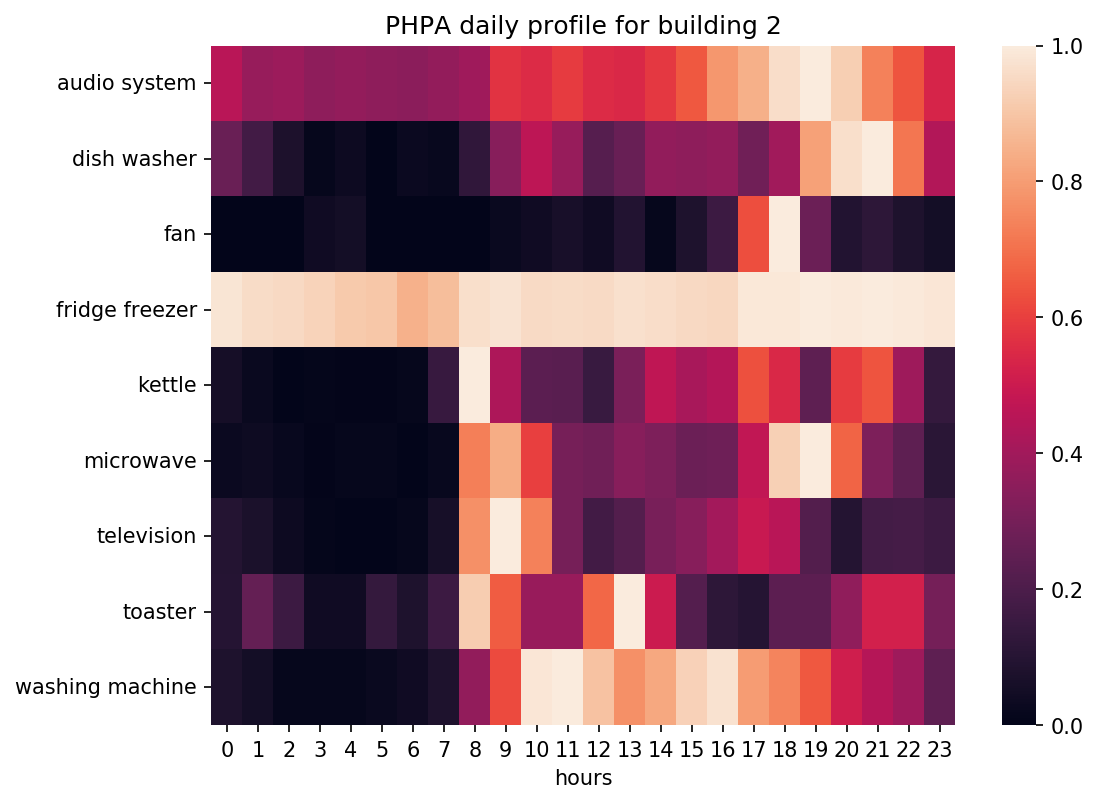
\includegraphics[width=1\linewidth]{../Figures/LPS/PHPA.png}
		\label{fig:ec_PHPA}
	\end{subfigure}%
	~ 
	\begin{subfigure}{.5\textwidth}
		% \centering
		\caption{"figure \protect\ref{arr:act_mat} as an image"}
		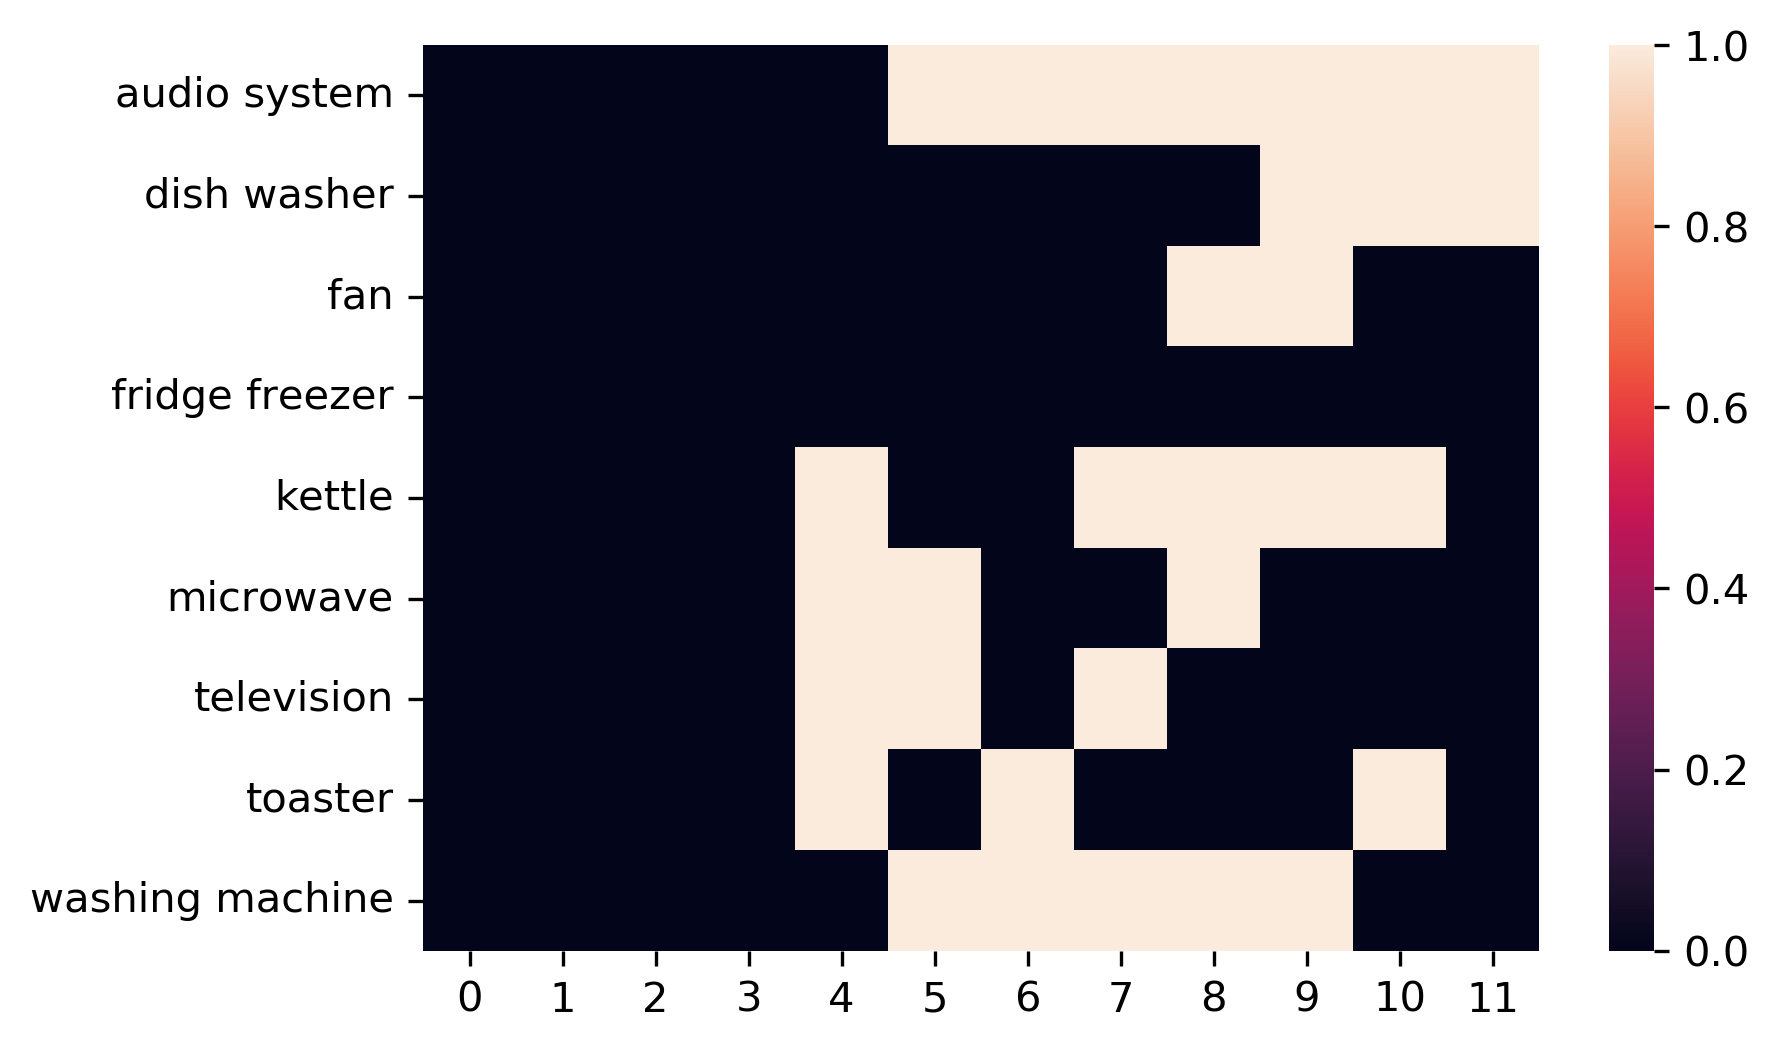
\includegraphics[width=1\linewidth]{../Figures/LPS/PHPA_EC.png}
		\label{fig:ec_PHPA_bw}
	\end{subfigure}%

	\caption{"Trasformation of source load profile to black and white"}
\end{figure}

\subsubsection{Step four}

Using the matrix \ref{arr:act_mat} we can write an algorithm that will use current activations 
and compare it to the matrix. For example, if we have the test sample for the fifth bucket, that is 
data from 8 to 10 o clock. 
What needs to be done is to use the fifth column and multiply the current activations.
Then anomaly is detected based on a rule. That at least two appliances must be activated, for the bucket to be labeled as normal,
or else the bucket is labeled as anomalous. In this case, we sum the elements of an array and check if it is larger or equal to 2. 

% \begin{figure}[H]
%     \centering
%     \begin{tikzpicture}
%         \coordinate (s) at (0,5);
%         \foreach \num in {0, 0, 0, 0, 0, 0, 0, 1, 1, 1, 1, 0}{
%         \node[minimum size=6mm, draw, rectangle] at (s) {\num};
%         \coordinate (s) at ($(s) + (1,0)$);
%         }
        
%         \node at (5.5,4) {X};
%         \coordinate (s) at (0,3);
%         \foreach \num in {1, 0, 0, 0, 0, 0, 0, 1, 0, 0, 1, 0}{
%         \node[minimum size=6mm, draw, rectangle] at (s) {\num};
%         \coordinate (s) at ($(s) + (1,0)$);
%         }
%         \node at (5.5,2){=};
%         \coordinate (s) at (0,1);
%         \foreach \num in {0, 0, 0, 0, 0, 0, 0, 1, 0, 0, 1, 0}{
%         \node[minimum size=6mm, draw, rectangle] at (s) {\num};
%         \coordinate (s) at ($(s) + (1,0)$);
%         }
%         \node at (5.5,0){SUM = 2 - > not an anomaly };
%     \end{tikzpicture}
%     \caption{The evaluation of new bucket compared to matrix. Example is for fifth bucket or fifth row from the matrix}
%     %\label{arr:microwave_acts_vec}
% \end{figure}

\begin{figure}[H]
    \centering
    \caption{"Process of evaluating an anomaly"}
    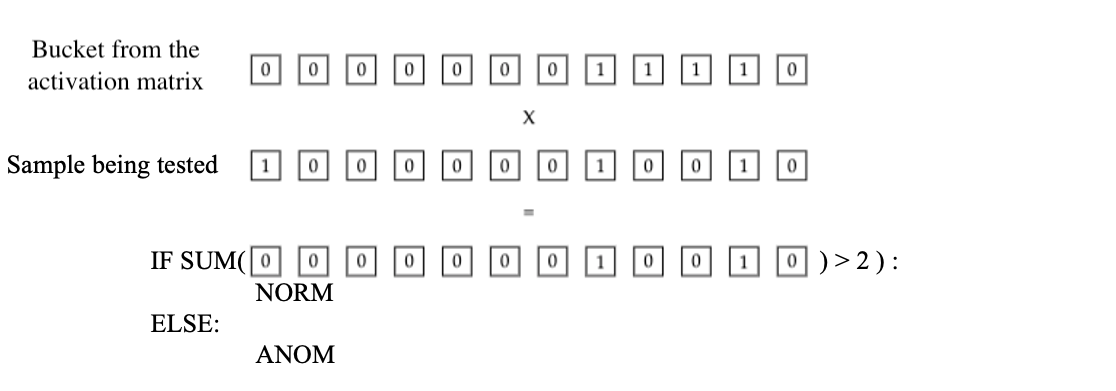
\includegraphics[width=1\linewidth]{../Figures/EC/EC_anom_dect.png}
    \label{fig:anom_detct}
    \caption{The evaluation of new bucket compared to matrix. Example is for fifth bucket or fifth row from the matrix}
    
\end{figure}

This process is done for all samples, where we count normal and anomalous samples for each bucket
The important thing to note here is that we are evaluating the samples from which the profile was built.

\begin{figure}[H]
    \centering
    \begin{tikzpicture}
        \coordinate (s) at (0,0);
        \foreach \num in {472, 469, 468, 466, 57, 153, 288, 187, 123, 84, 75, 281}{
        \node[minimum size=6mm, draw, rectangle] at (s) {\num};
        \coordinate (s) at ($(s) + (1,0)$);
        }
    \end{tikzpicture}
    \caption{Agregated anomalies for each bucket}
    \label{arr:agg_anom}
\end{figure}

\begin{figure}[H]
    \centering
    \begin{tikzpicture}
        \coordinate (s) at (0,0);
        \foreach \num in {0, 0, 0, 0, 409, 312, 181, 280, 342, 384, 394, 188}{
        \node[minimum size=6mm, draw, rectangle] at (s) {\num};
        \coordinate (s) at ($(s) + (1,0)$);
        }
    \end{tikzpicture}
    \caption{Agregated normal samples for each bucket}
    \label{arr:agg_norm}
\end{figure}

The next step is to combine these two arrays so that we calculate the percentage of anomalous samples 
for each bucket with an equation

\begin{equation}
    a / (a + n) 
\end{equation}

Where "a" is a number of anomalous samples and "n" is a number of normal samples.

\begin{figure}[H]
    \centering
    \begin{tikzpicture}
        \coordinate (s) at (0,0);
        \foreach \num in {1.0, 1.0, 1.0, 1.0, 0.12, 0.3, 0.61, 0.4, 0.26, 0.18, 0.16, 0.6}{
        \node[minimum size=6mm, draw, rectangle] at (s) {\num};
        \coordinate (s) at ($(s) + (1,0)$);
        }
    \end{tikzpicture}
    \caption{Agregated anomalies for each bucket}
    \label{arr:anom_ratio}
\end{figure}

In other words, the \ref{arr:anom_ratio} tells us how persistent is the user's routine in each bucket or
part of the day. The lower the ratio the higher the routine. Since routine is detected based on the usage
of appliances it cannot be picked up during the night. It is possible to see that the routine is quite high 
during the morning and evening hours. The anomaly detection algorithm will work best when the ratio above is low.
A good trait of elders is that their routine is quite high even during the day, which means that
the anomaly detection will function better throughout the day.

One more thing to do is to ignore the parts of the day when the user has no routine, by using
the array \ref{arr:anom_ratio} and setting a threshold of 0.3. A threshold of 0.5 would mean
that every other day could be a false positive anomaly. Setting the rate at 0.3 reduces that 
to every third day. But here compromises must be made, the lower the threshold the more accurate
the algorithm will be, but it also means that it will be less sensitive. 
In our case, there is not much harm in false positives detections, since the caregiver can call
the elder to check if it is okay.  

\begin{figure}[H]
    \centering
    \begin{tikzpicture}
        \coordinate (s) at (0,0);
        \foreach \num in {0, 0, 0, 0, 1, 1, 0, 0, 1, 1, 1, 0}{
        %\foreach \num in {1.0, 1.0, 1.0, 1.0, 0.12, 0.3, 0.61, 0.4, 0.26, 0.18, 0.16, 0.6}{
        \node[minimum size=6mm, draw, rectangle] at (s) {\num};
        \coordinate (s) at ($(s) + (1,0)$);
        }
    \end{tikzpicture}
    \caption{Using above-mentioned threshold a new mask is made, to check only buckets with high routine}
    \label{arr:anom_ratio_mask}
\end{figure}

\subsubsection{Step five}

The last step is to repeat steps 4 and 5 with data, that is not included in the built profile.

\subsection{Datasets and evaluation} \label{ssec:ds_eval}

The data was split into train and test sets, where 80 \% of the data was for training and 20 \% percent of the data was used for testing.
The data was split based on the number of samples, so in some cases where there is a lot of missing data, the time window of test data might be longer, although it contains only 20 \% of the samples.
\subsubsection{REFIT}
The REFIT dataset included data for more than 15 buildings, as can be seen on the figure below.
The dataset in general is of the highest quality since it is the longest. This means this dataset should give the most relevant results.
\begin{figure}[H]
	\centering
	\caption{"Timeline for REFIT "}
	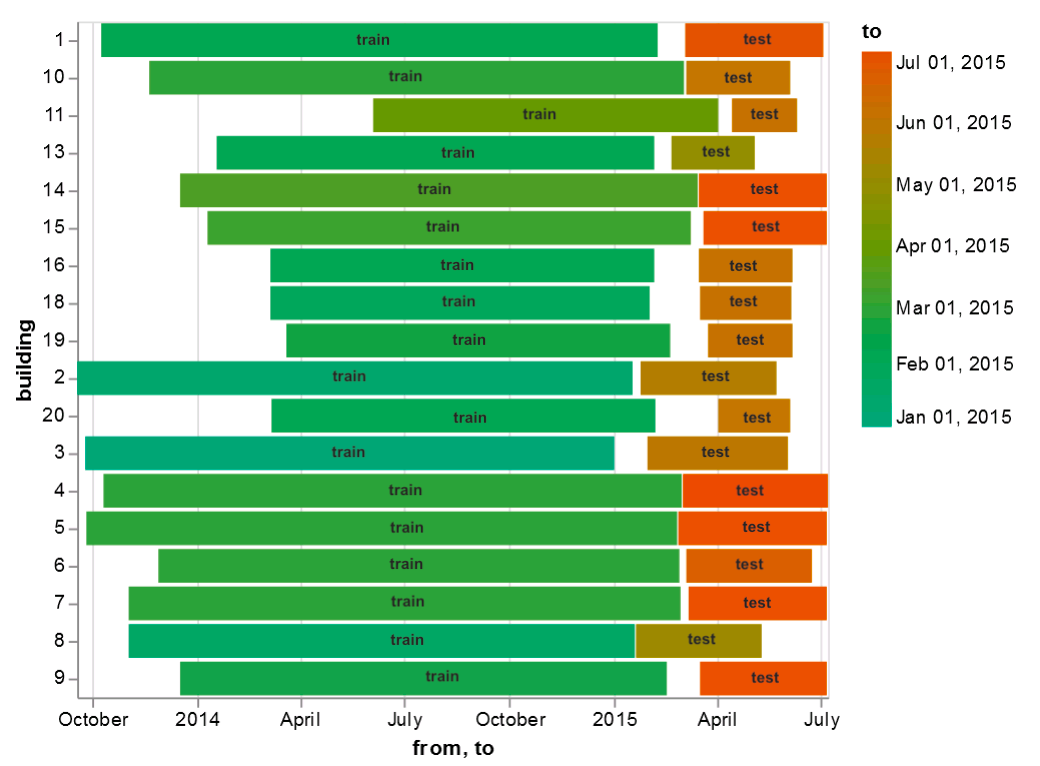
\includegraphics[width=1\textwidth]{Figures/EC/refit_timeline.png}
	\label{fig:refit_timeline}
\end{figure}
fd
\subsubsection{UK-DALE} 

All through the UK-DALE dataset is of similar size, the most of the data is from building 1.
In general, it includes 5 years of data, but only for some appliances, with addition, many appliances are rarely used.
When taking all of this into account, there are too many issues with it, and it was simply ignored.
Another issue that can be seen on \ref{fig:ukdale_timeline} is that there is not enough data for 
building 3. The test includes only a week of data, which is not enough for representative results, therefore it was ignored.
The rest of the buildings seem healthy.

\begin{figure}[H]
	\centering
	\caption{"Timeline for UK-DALE "}
	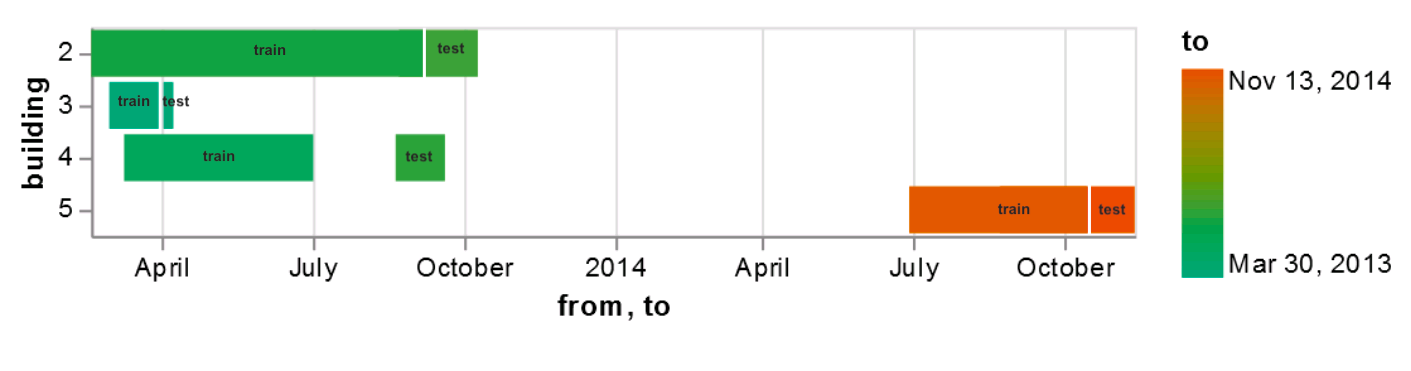
\includegraphics[width=1\textwidth]{Figures/EC/ukdale_timeline.png}
	\label{fig:ukdale_timeline}
\end{figure}

\subsubsection{ECO}
ECO dataset has a length of data, similar to UK-DALE. 
The only issue is building 1, where there is a lot of missing data.
This is a good example of how data is split, it is split based on several samples,
meaning that there is 80 \% in the train bar, due to missing data the second bar is longer. 

\begin{figure}[H]
	\centering
	\caption{"Timeline for ECO"}
	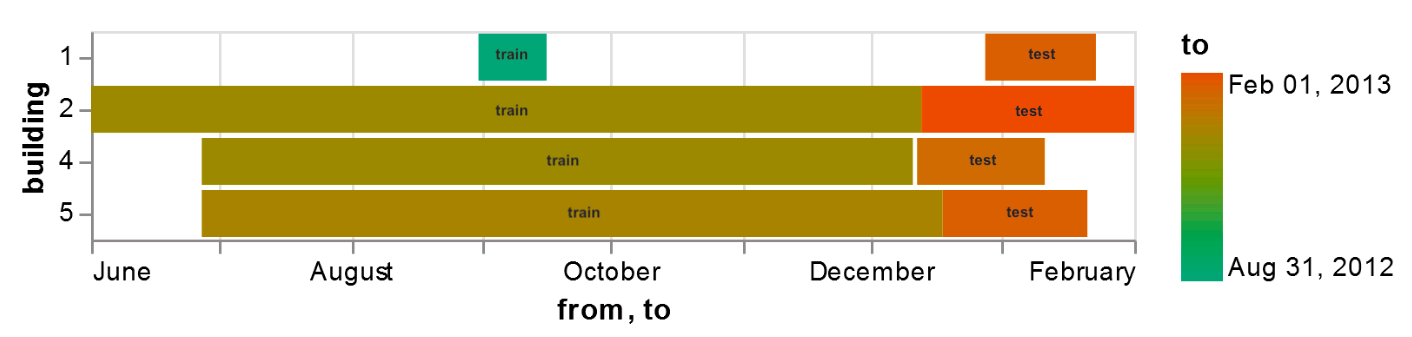
\includegraphics[width=1\textwidth]{Figures/EC/eco_timeline.png}
	\label{fig:eco_timeline}
\end{figure}


\subsection{The ratio}

Due to the lack of ground truth data of actual accidents, it is hard to determine the 
exact accuracy of this algorithm. Every anomaly detected is not necessarily an 
actual accident, it could be that the user decided to lie in bed a bit longer, or decided to go to bed early in the evening.
One metric that we can use to determine how well the algorithm functions is the anomaly ratio \ref{arr:anom_ratio}.
The reason behind that is, that if the routine rate is high it means that it will be easier to detect.

\begin{itemize}
	\item ratio of 1 would mean that for that bucket household has no routine at all.
    \item ratio of 0.5 would mean that the routine is being "practiced" every second day
    \item ratio of 0.2 would mean that routine is broken on average every 5 day
    \item ratio of 0 would mean that this household has a routine that is never broken. 
\end{itemize}

When a true anomaly occurs such as a fall, the dweller, all through he had the same routine for the past year (the ratio would be close to 0), would not be able to practice the routine, and the algorithm will be quite sure that this is an actual anomaly.
Therefore, the higher the ratio the less sure we are that an actual anomaly such as a fall occurred.
This is a good alternative measurement, that tells us how well this algorithm will perform. 

\subsubsection{Ratio during the week} \label{sssec:ratio_week}

As the behavior of the dweller's changes, so does the accuracy of the algorithm. 
One observation that was made, was that the routine was higher during the week than during the weekends,
as can be seen in the figures below. There is also a 

\begin{figure}[H]
	\begin{subfigure}{.5\textwidth}
		% \centering
		\caption{"Building 2"}
		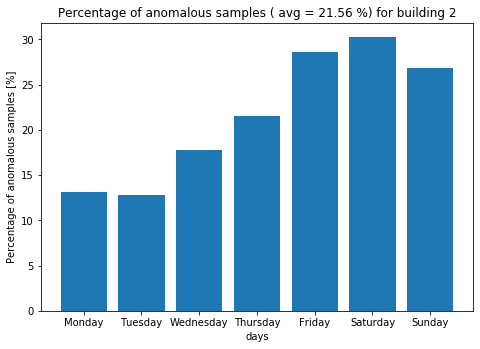
\includegraphics[width=1\linewidth]{../Figures/EC/b2week.png}
		\label{fig:ec_b2week}
	\end{subfigure}%
	~ 
	\begin{subfigure}{.5\textwidth}
		% \centering
		\caption{"Building 19"}
		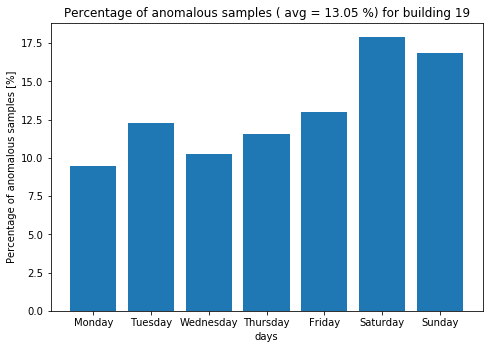
\includegraphics[width=1\linewidth]{../Figures/EC/b19week.png}
		\label{fig:ec_b5week}
	\end{subfigure}%
    \bigskip

    \begin{subfigure}{.5\textwidth}
		% \centering
		\caption{"Building 18"}
		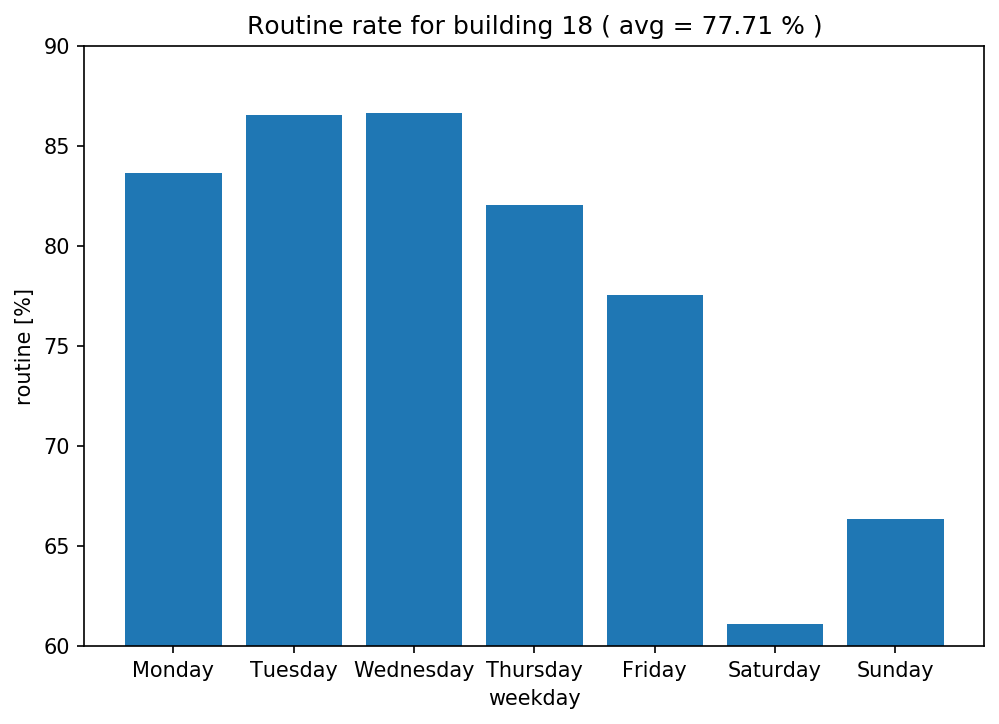
\includegraphics[width=1\linewidth]{../Figures/EC/b18week.png}
		\label{fig:ec_b18week}
	\end{subfigure}%
    ~ 
    \begin{subfigure}{.5\textwidth}
		% \centering
		\caption{"Building 5"}
		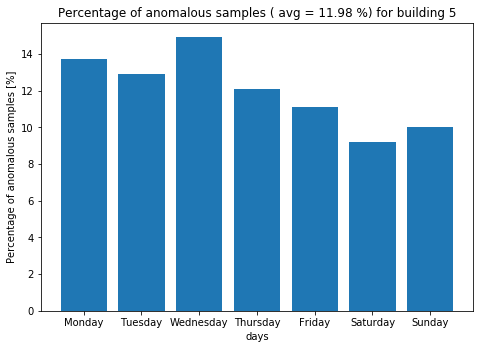
\includegraphics[width=1\linewidth]{../Figures/EC/b5weekd.png}
		\label{fig:ec_b5week}
	\end{subfigure}%
	\label{fig:ec_week}
	\caption{"Weekly anomaly percenage"}
\end{figure}

Since we are dealing with the elderly, they have a higher routine, and it does not change that much during the weekends. 
Usually, assisted living systems are put in place since elders are alone in the dwelling.
Taking all of this into account, we could assume that the routine of the elderly is the same trough the week and simply ignore the weekends. 
This should yield more relevant results. 

\subsection{Ratio in a year}

The ratio also changes over a year. While on average the ratio is lower during the winter, spring and summer, it is higher during the summer due to vacation. 
This can be seen in the figures below. 

\begin{figure}[H]
	\begin{subfigure}{.5\textwidth}
		% \centering
		\caption{"Building 2"}
		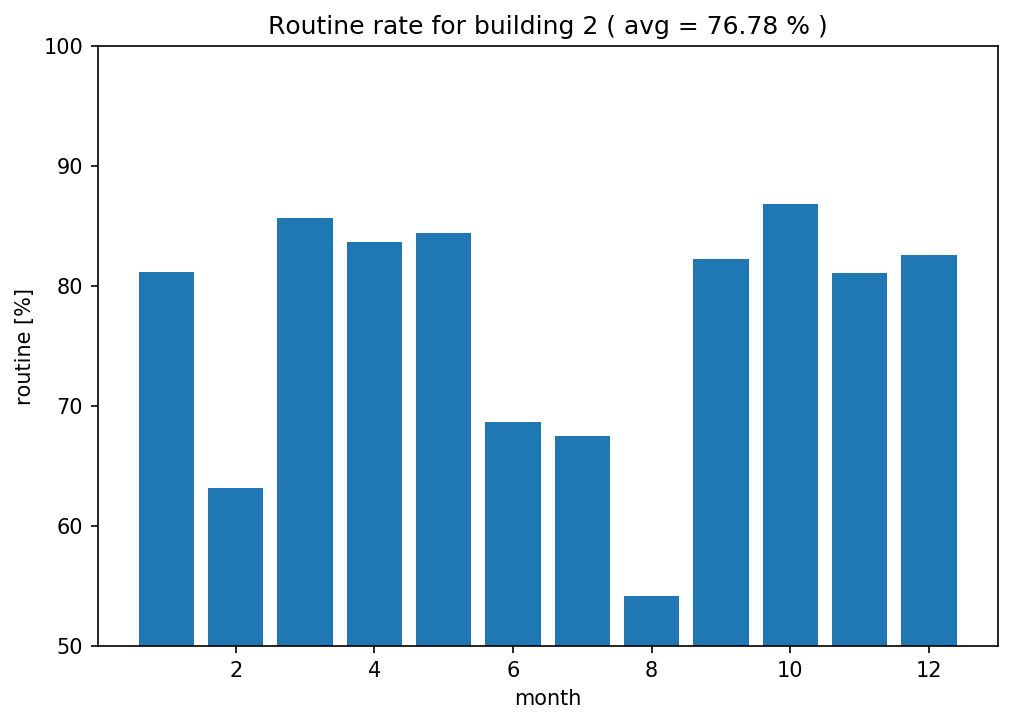
\includegraphics[width=1\linewidth]{../Figures/EC/b2year.png}
		\label{fig:ec_b2year}
	\end{subfigure}%
	~ 
	\begin{subfigure}{.5\textwidth}
		% \centering
		\caption{"Building 19"}
		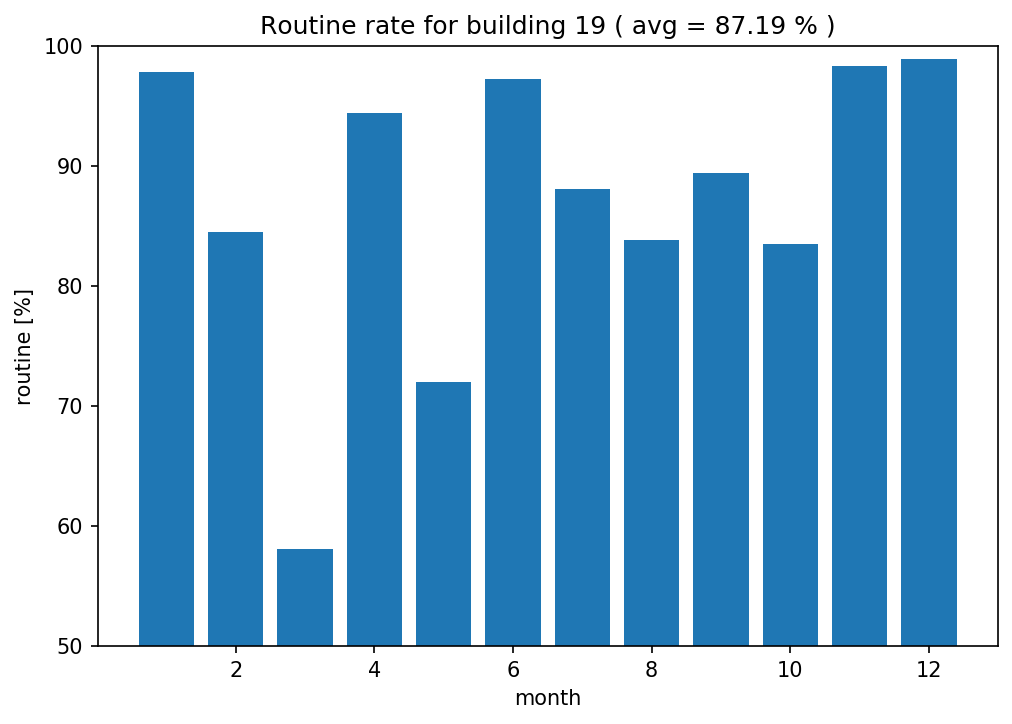
\includegraphics[width=1\linewidth]{../Figures/EC/b19year.png}
		\label{fig:ec_b5year}
	\end{subfigure}%
    \bigskip

    \begin{subfigure}{.5\textwidth}
		% \centering
		\caption{"Building 18"}
		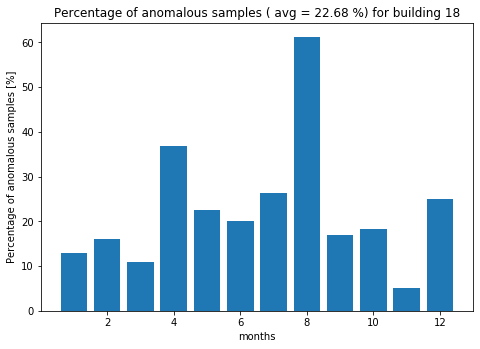
\includegraphics[width=1\linewidth]{../Figures/EC/b18year.png}
		\label{fig:ec_b18year}
	\end{subfigure}%
    ~ 
    \begin{subfigure}{.5\textwidth}
		% \centering
		\caption{"Building 5"}
		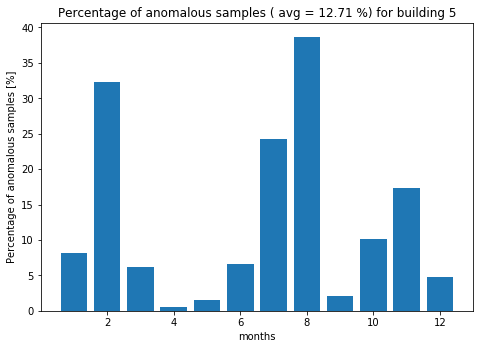
\includegraphics[width=1\linewidth]{../Figures/EC/b5year.png}
		\label{fig:ec_b5year}
	\end{subfigure}%
	\label{fig:ec_year}
	\caption{"Yearly anomaly percentage"}
\end{figure}

\subsection{Effectivness of anomaly detection}

One more thing to keep in mind is that this algorithm will be able to detect anomalies only when
the routine will be high, and more than two appliances will be used in that buckets.

add example here

Figure \ref{fig:ignored_buckets_22} shows which buckets were most commonly used for the detection of an anomaly.
The graph includes averaged values from all buildings and datasets. 
In other words, the graph presents how strong is average routine through the day.

This means that the higher the percentage, the higher the chance that this bucket will be usable.
During the night, it is possible to see that the average routine rate is quite high,
this is because most users are routinely sleeping during that period. 
As said this high percentage enables us to detect possible accidents while sleeping.
Should the elder wake up due to a problem, it could be detected.
In case if elder wakes up during the night, it would be hard to detect it, since the algorithm would think it is part of the routine.

\begin{figure}[H]
	\centering
	\caption{"Percentage of buildings that used bucket for anomaly detection"}
	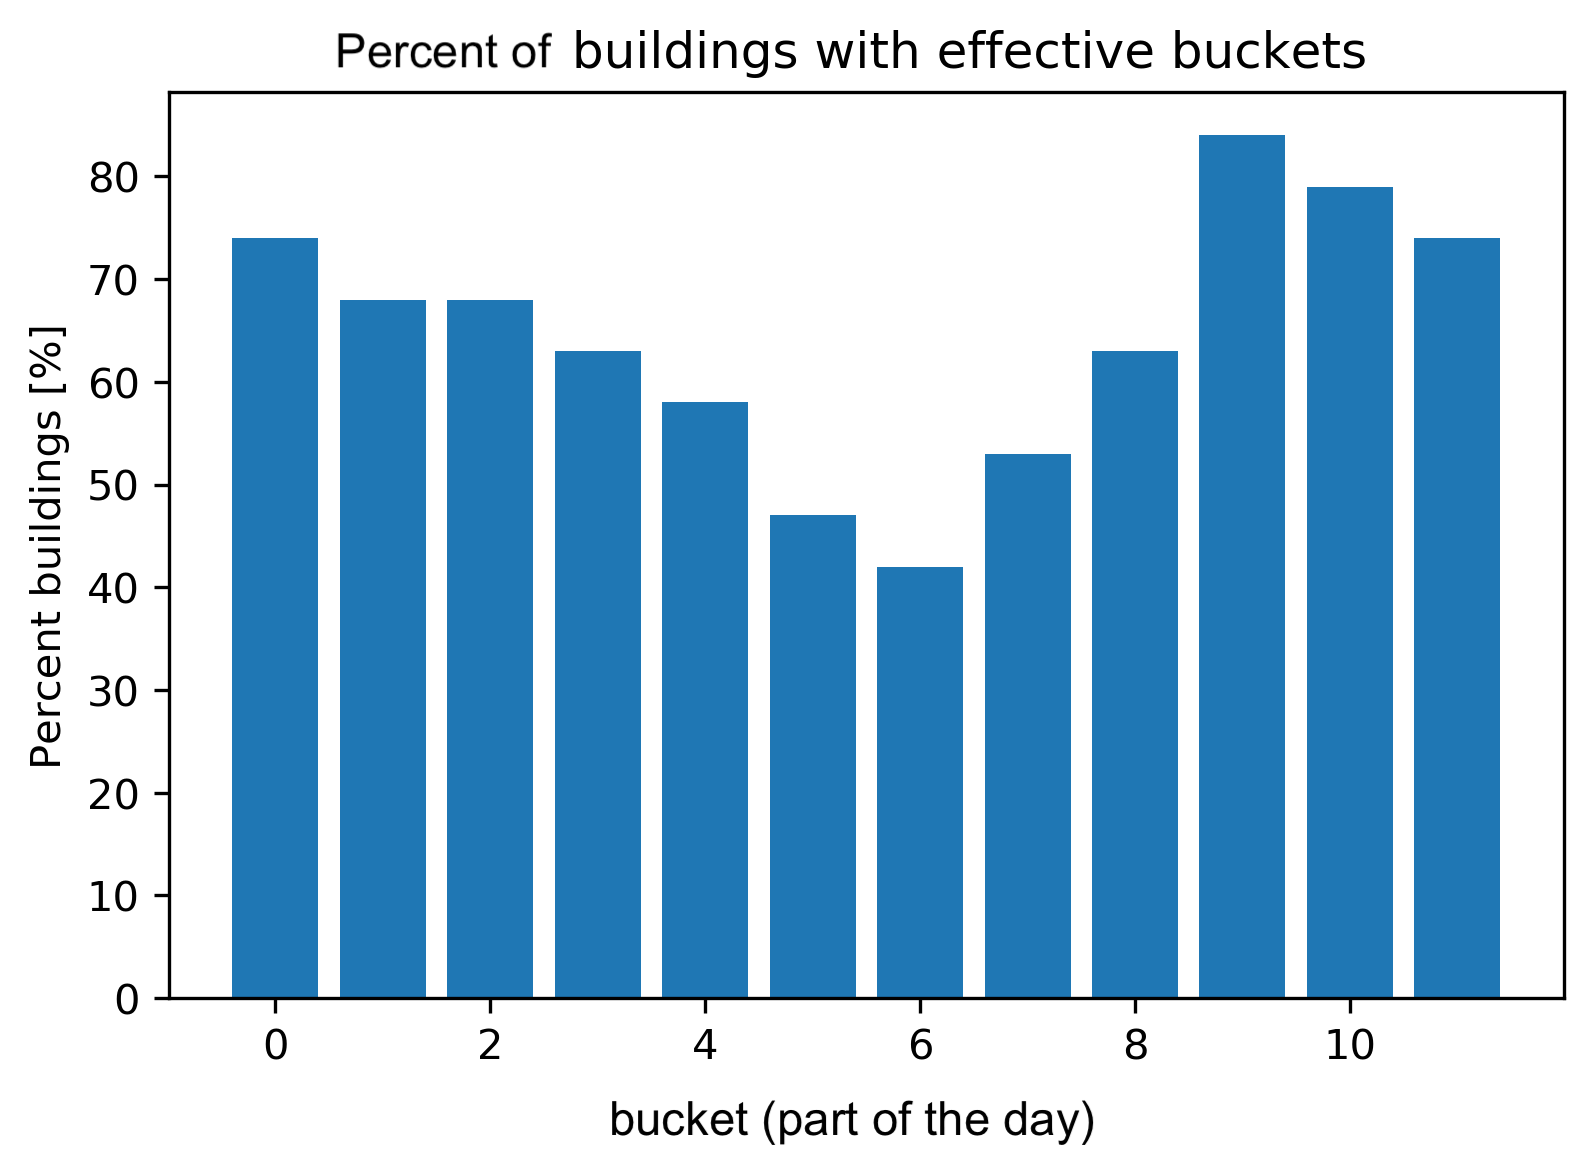
\includegraphics[width=.8\textwidth]{Figures/EC/ignored_buckets_dist.png}
	\label{fig:ignored_buckets_22}
\end{figure}

To find the most usable buckets for our operating mode, an additional filter must be applied.
The rule is that at least two appliances must be commonly used in that bucket. 
After applying this rule the following figure emerges \ref{fig:ignored_buckets_act}

\begin{figure}[H]
	\centering
	\caption{"Percentage of buildings that used effetive buckets for anomaly detection "}
	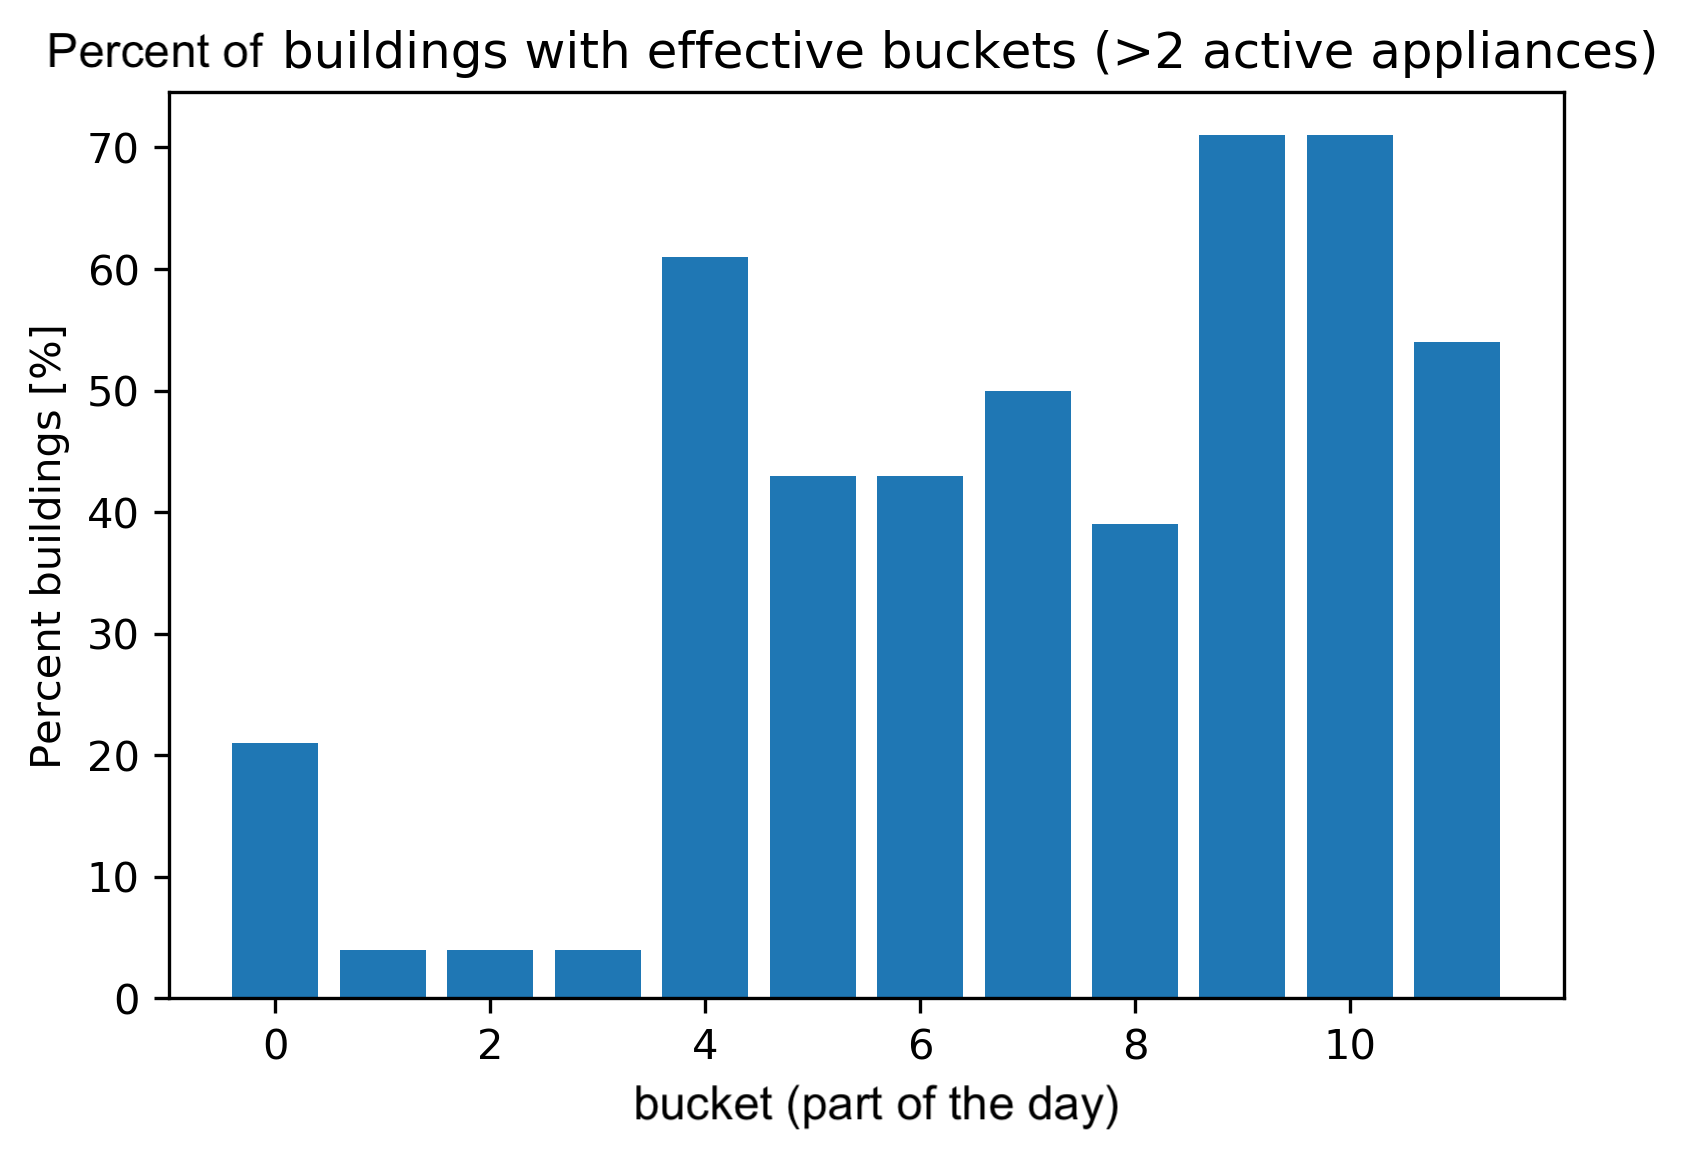
\includegraphics[width=.8\textwidth]{Figures/EC/all_ignored_buckets_dist_incl_act.png}
	\label{fig:ignored_buckets_act}
\end{figure}

The figure \ref{fig:ignored_buckets_act} shows that there are two peaks.
One in the morning and the other, a wider one in the evening.

This means that on an average home the algorithm would perform best in the morning and evening.
This is because the average person is at school or work during noon. 
This can be confirmed on figure \ref{fig:ignored_buckets_act}.
The elderly, are usually at home at noon, which could extend the effective detection window.

\section{Results}

The examples above were a demonstration and a look into data and metrics. 
The examples shown were trained and evaluated on the same data. 
To show true performance, we will use test data to determine the actual performance. 

Results were obtained for 3 datasets. 
REDD and iAWE datasets were not used, since the dataset was too short, they contained less than a month of data. 


\subsection{REFIT}

\subsubsection{Results including weekend data}
Results show, that the method is on average 23.6 \% efficient. 
In figure \ref{fig:refit_res} it is possible to see that house 6 yields lower results and house 19 is much higher than the rest. 
This could be due to various dataset errors that occurred during sampling.

\begin{figure}[H]
	\centering
	\caption{"Results for REFIT "}
	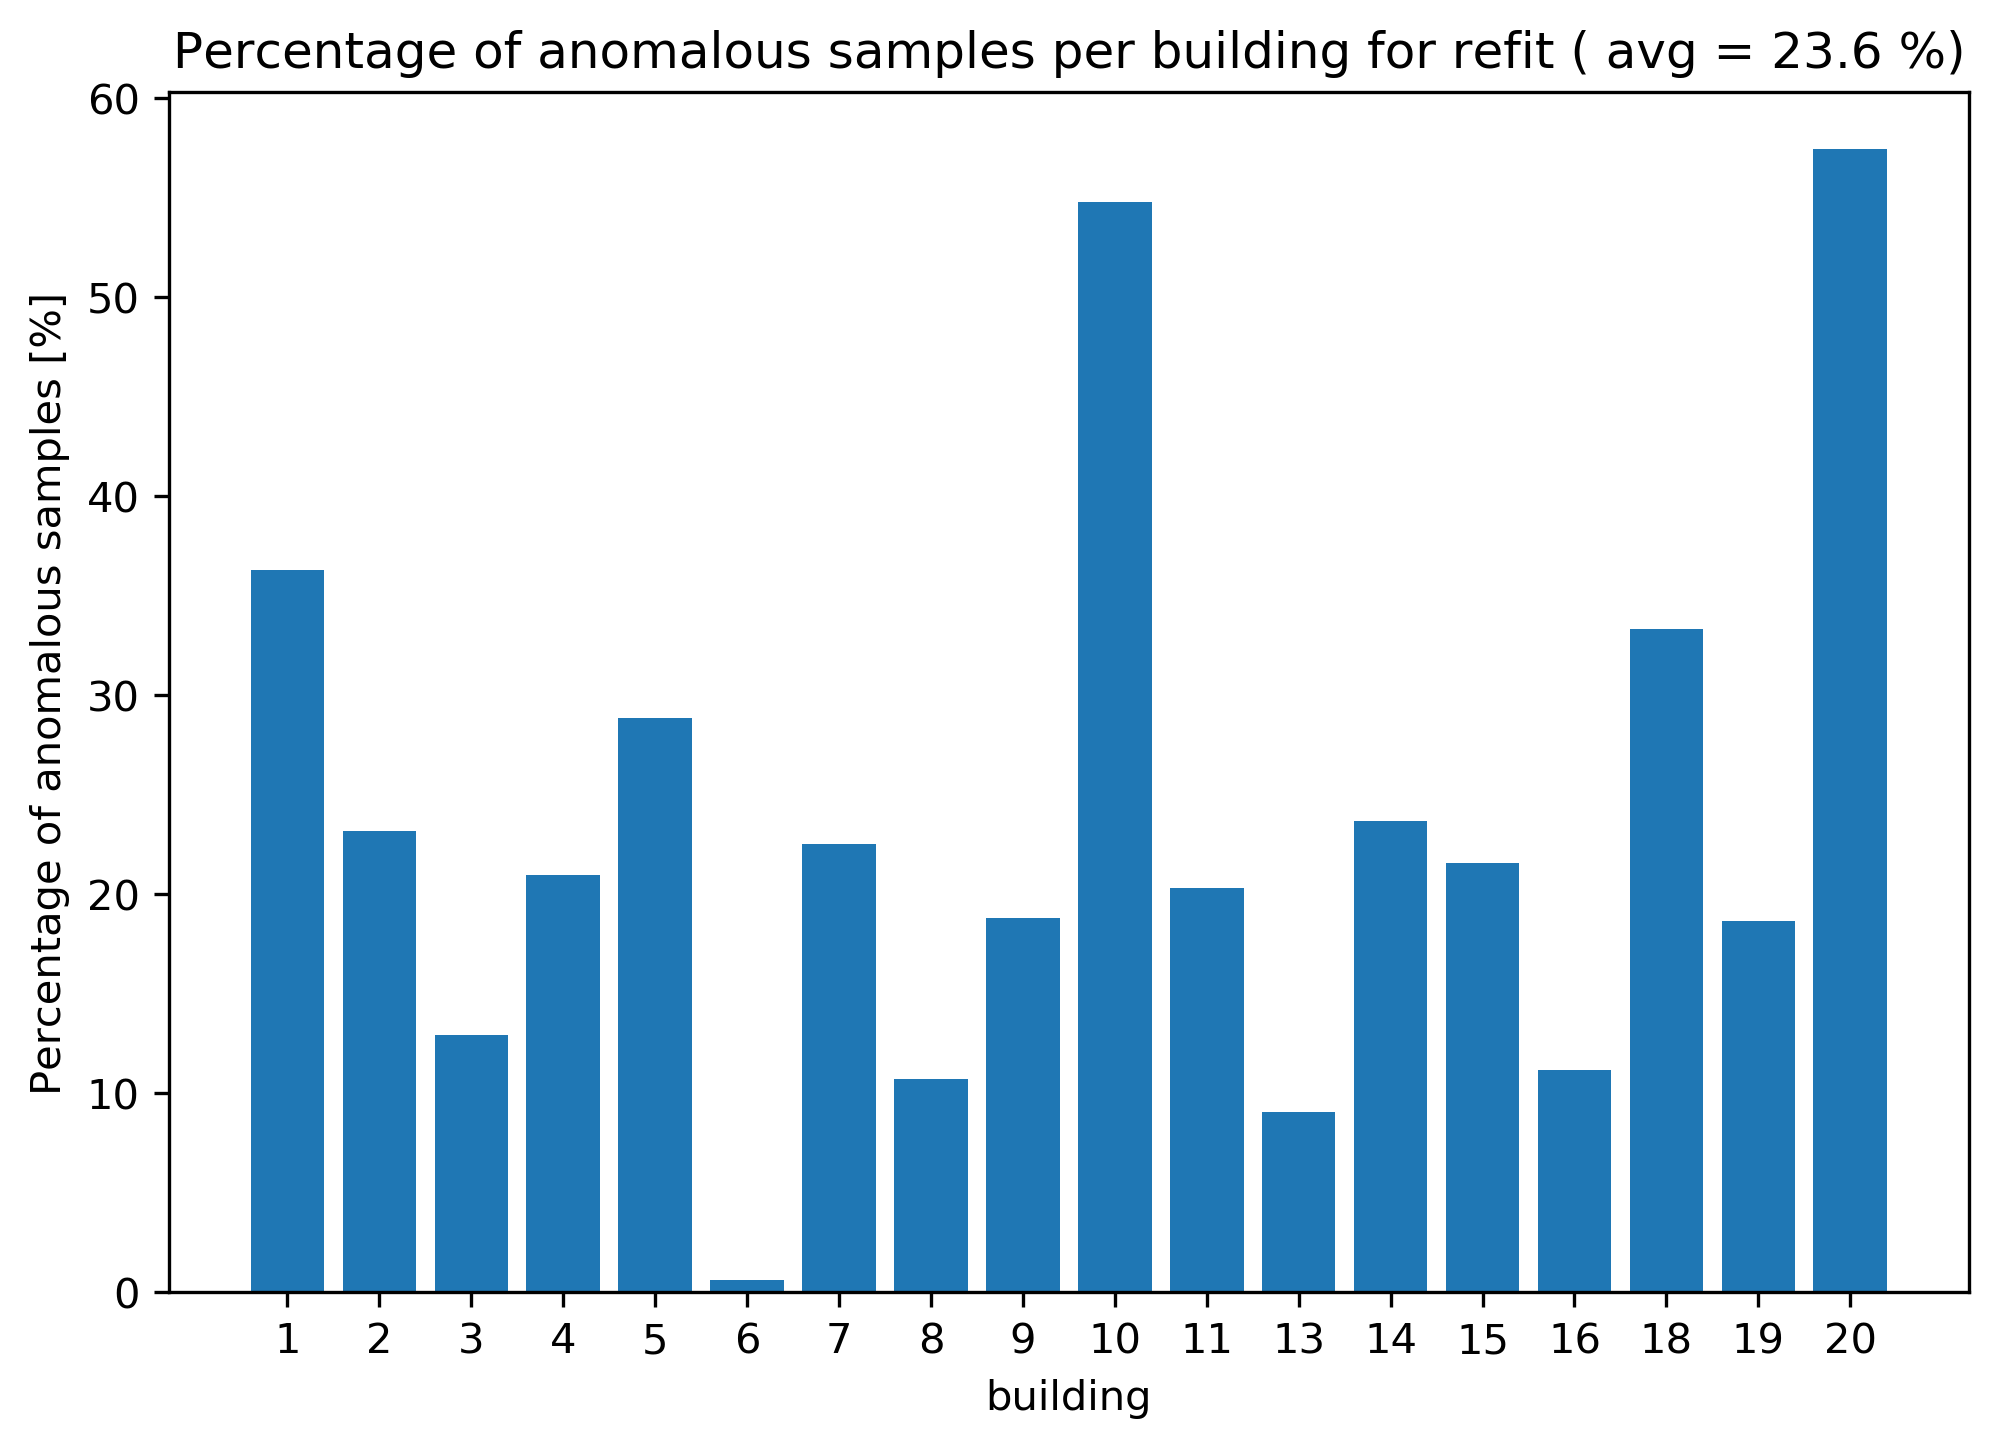
\includegraphics[width=.8\textwidth]{Figures/EC/refit_res.png}
	\label{fig:refit_res}
\end{figure}

For more relevant results we can ignore the outliers by removing one maximum and minimum value, such as can be seen in figure \ref{fig:refit_res2}
This yields a result of 22.92 \%.
If we were to repeat this process the result would be 21.33 \%.
Since all outliers are removed, the result converges towards 21 \%, which is the relevant value. 

\begin{figure}[H]
	\centering
	\caption{"Results for REFIT with removed outliers "}
	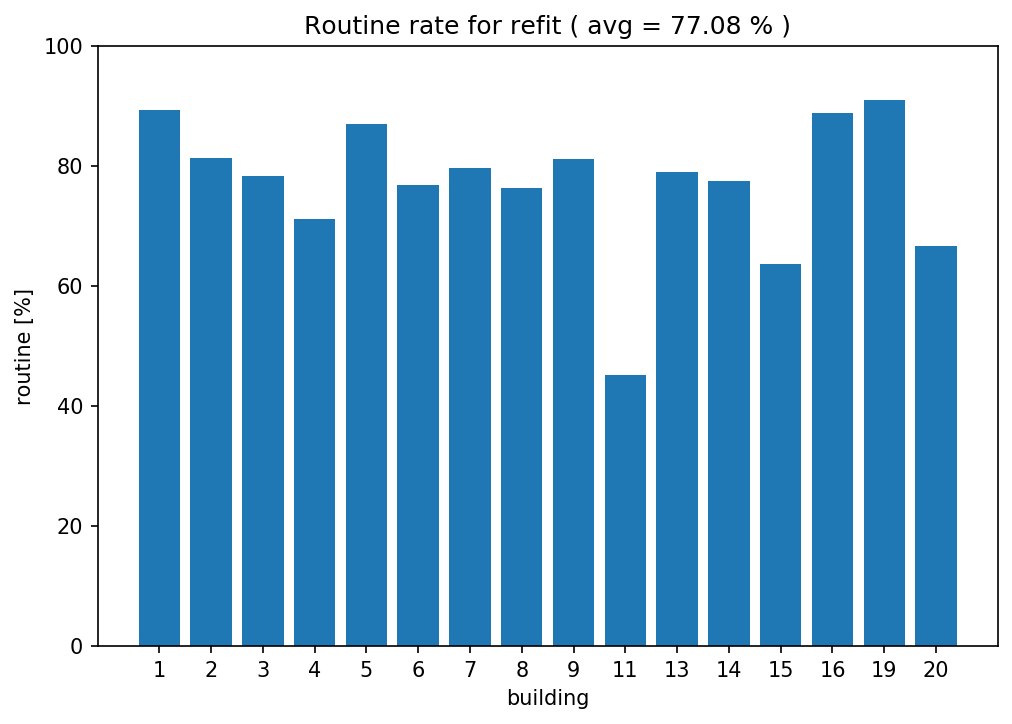
\includegraphics[width=.8\textwidth]{Figures/EC/refit_res2.png}
	\label{fig:refit_res2}
\end{figure}

\subsubsection{Omiting weekend data}

As mentioned in the sub-sub section \ref{sssec:ratio_week}, the average routine is different during the week and weekends.
The assumption was that the routine of elderly people does not change significantly over the week, therefore results should be more relevant if we ignore the weekends.
The results on figure \ref{fig:refit_res_nw_1"} show that result dropped to 22.48 \%.

\begin{figure}[H]
	\centering
	\caption{"Results for REFIT weekday only"}
	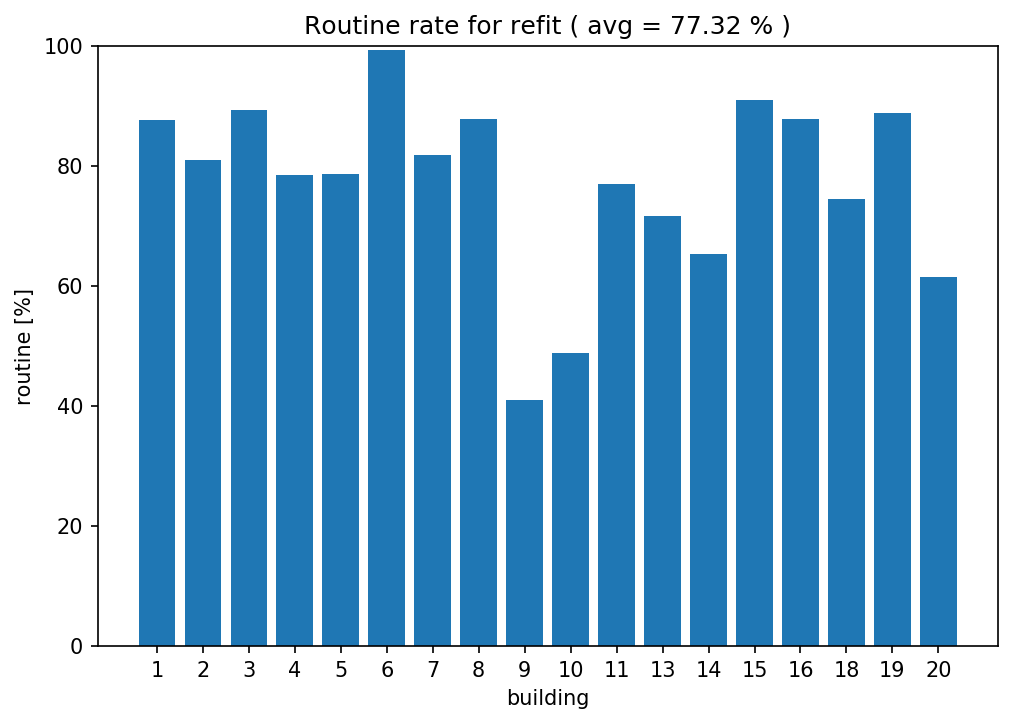
\includegraphics[width=.8\textwidth]{Figures/EC/refit_res_nw_1.png}
	\label{fig:refit_res_nw_1"}
\end{figure}

By ignoring the minimal and maximal outliers the results drop to 21.33 \%.
By repeating the process one more time the result drops to 19.91 \%, since all outliers were removed, the result converges towards this value. 

By removing the weekend data, the results decreased by 1.2 \%. 

\begin{figure}[H]
	\centering
	\caption{"Results for REFIT weekday only and removed outliers"}
	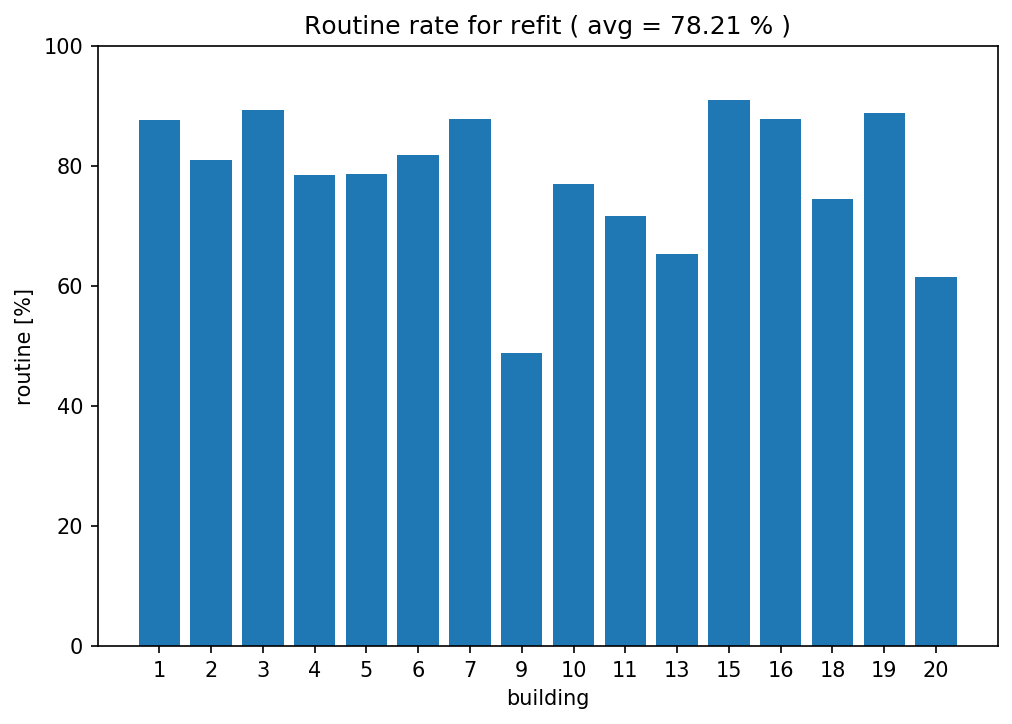
\includegraphics[width=.8\textwidth]{Figures/EC/refit_res_nw_2.png}
	\label{fig:refit_res_nw_2"}
\end{figure}

\subsection{UK-DALE}

As mentioned in subsection \ref{ssec:ds_eval}, the UK-DALE is not as long, large and cleaned as the previous dataset, so results could be less relevant.
The results on figure \ref{fig:ukdale_res}, show that the average result is 25.35 \%. Due to the low number of buildings, it is not possible to detect and ignore outliers.

\begin{figure}[H]
	\centering
	\caption{"Results for UK-DALE"}
	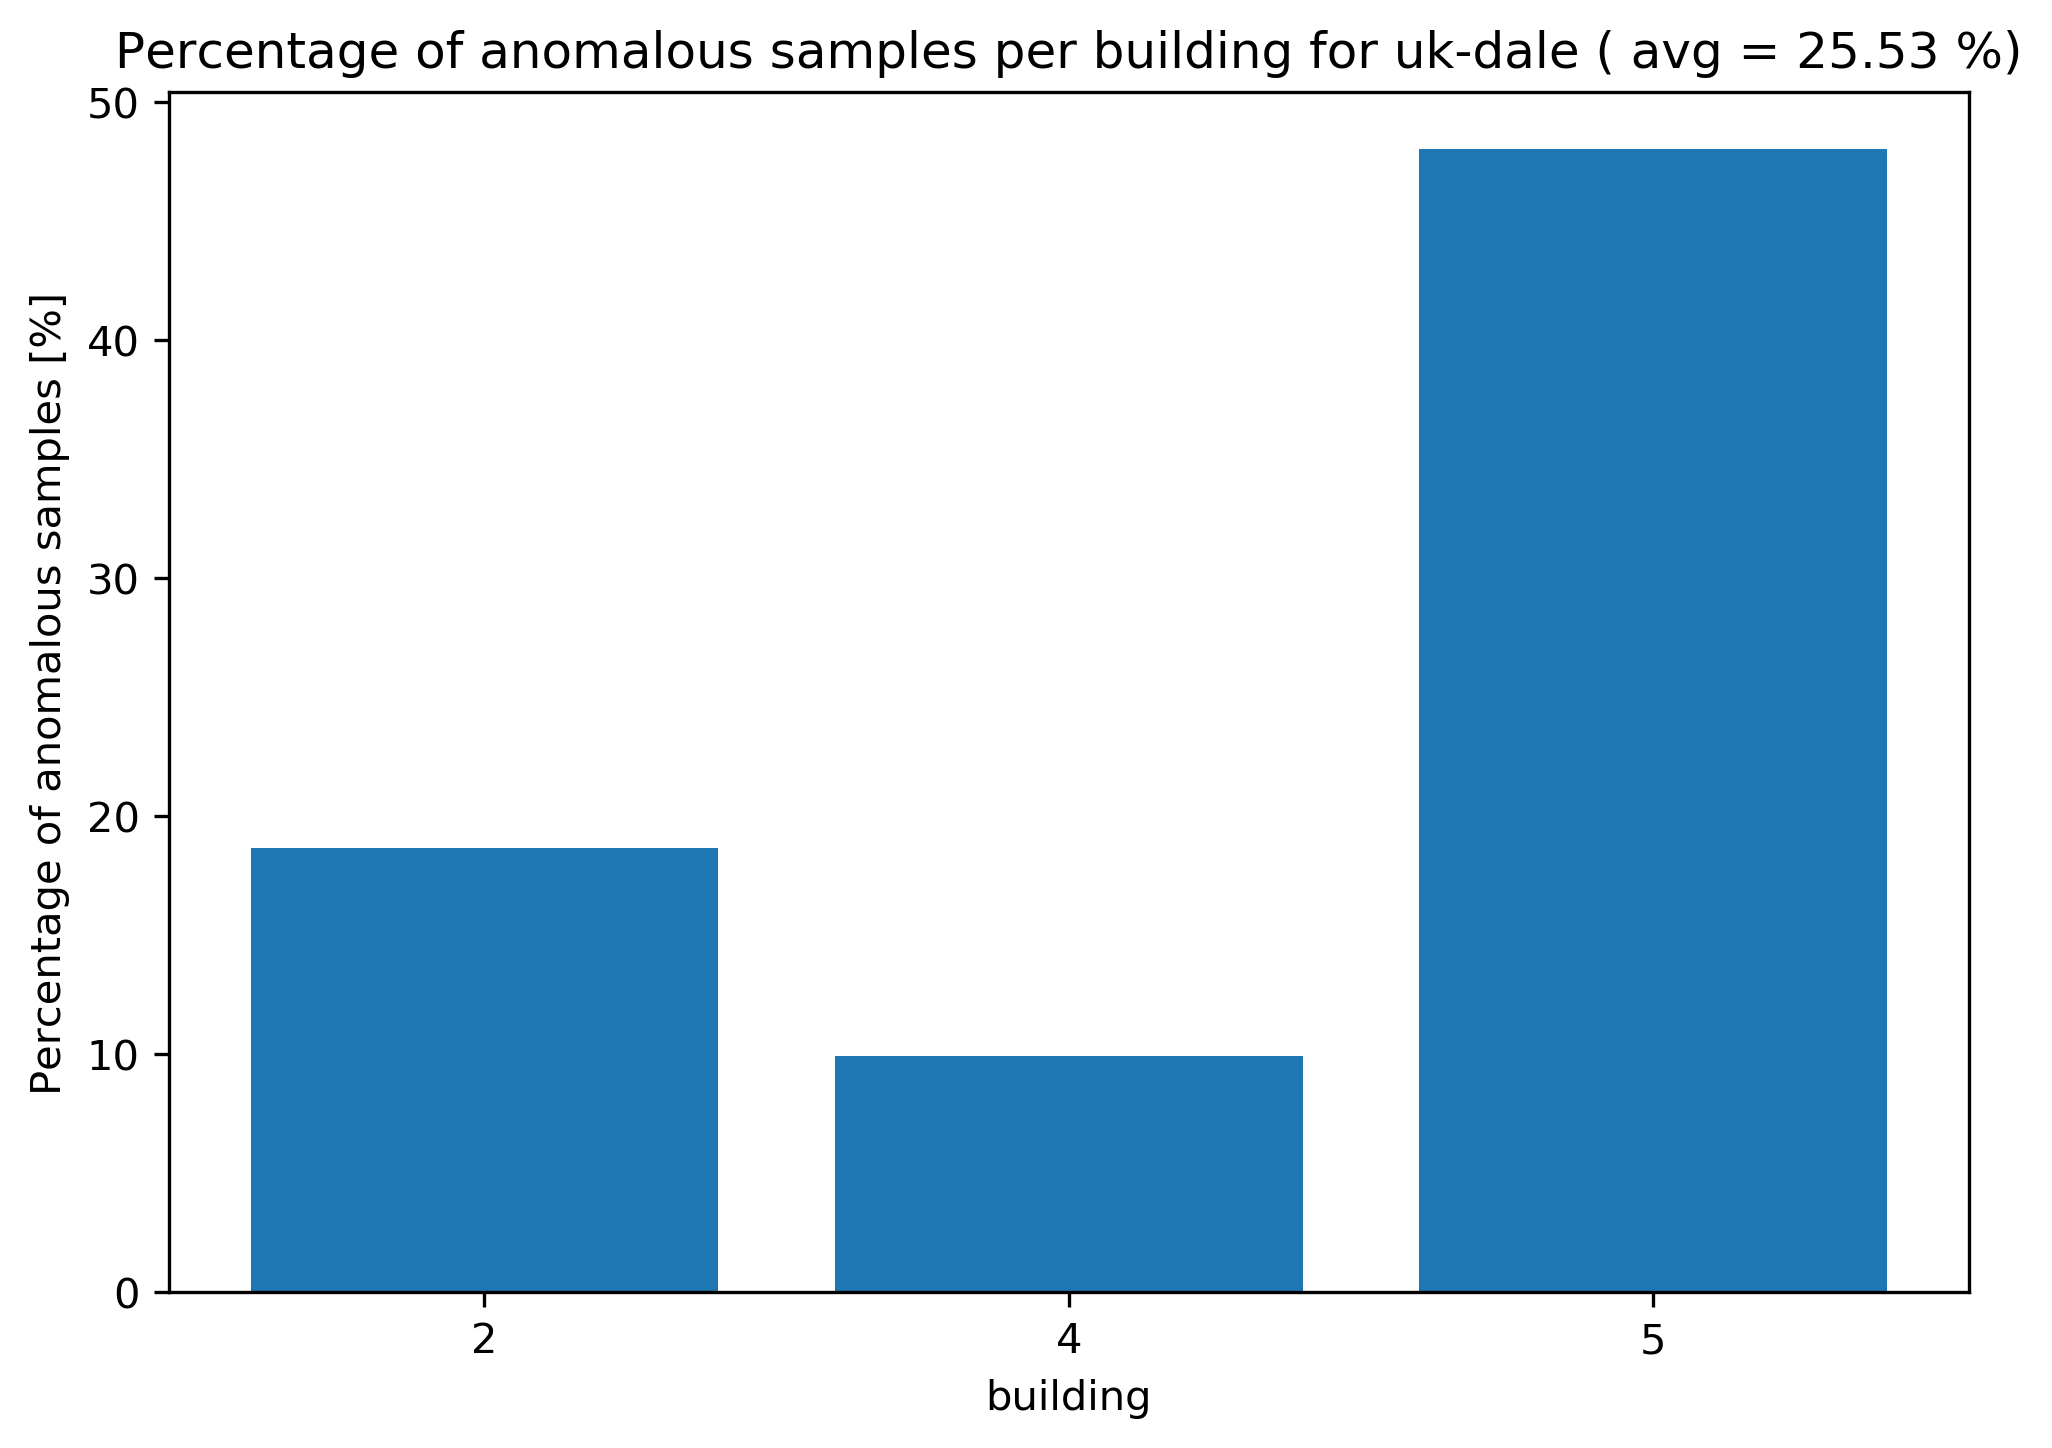
\includegraphics[width=.7\textwidth]{Figures/EC/ukdale_res.png}
	\label{fig:ukdale_res}
\end{figure}

The same as for REFIT, the weekend data can be ignored,
In this case, this does not improve the result. 

\begin{figure}[H]
	\centering
	\caption{"Results for UK-DALE omitinng weekends  "}
	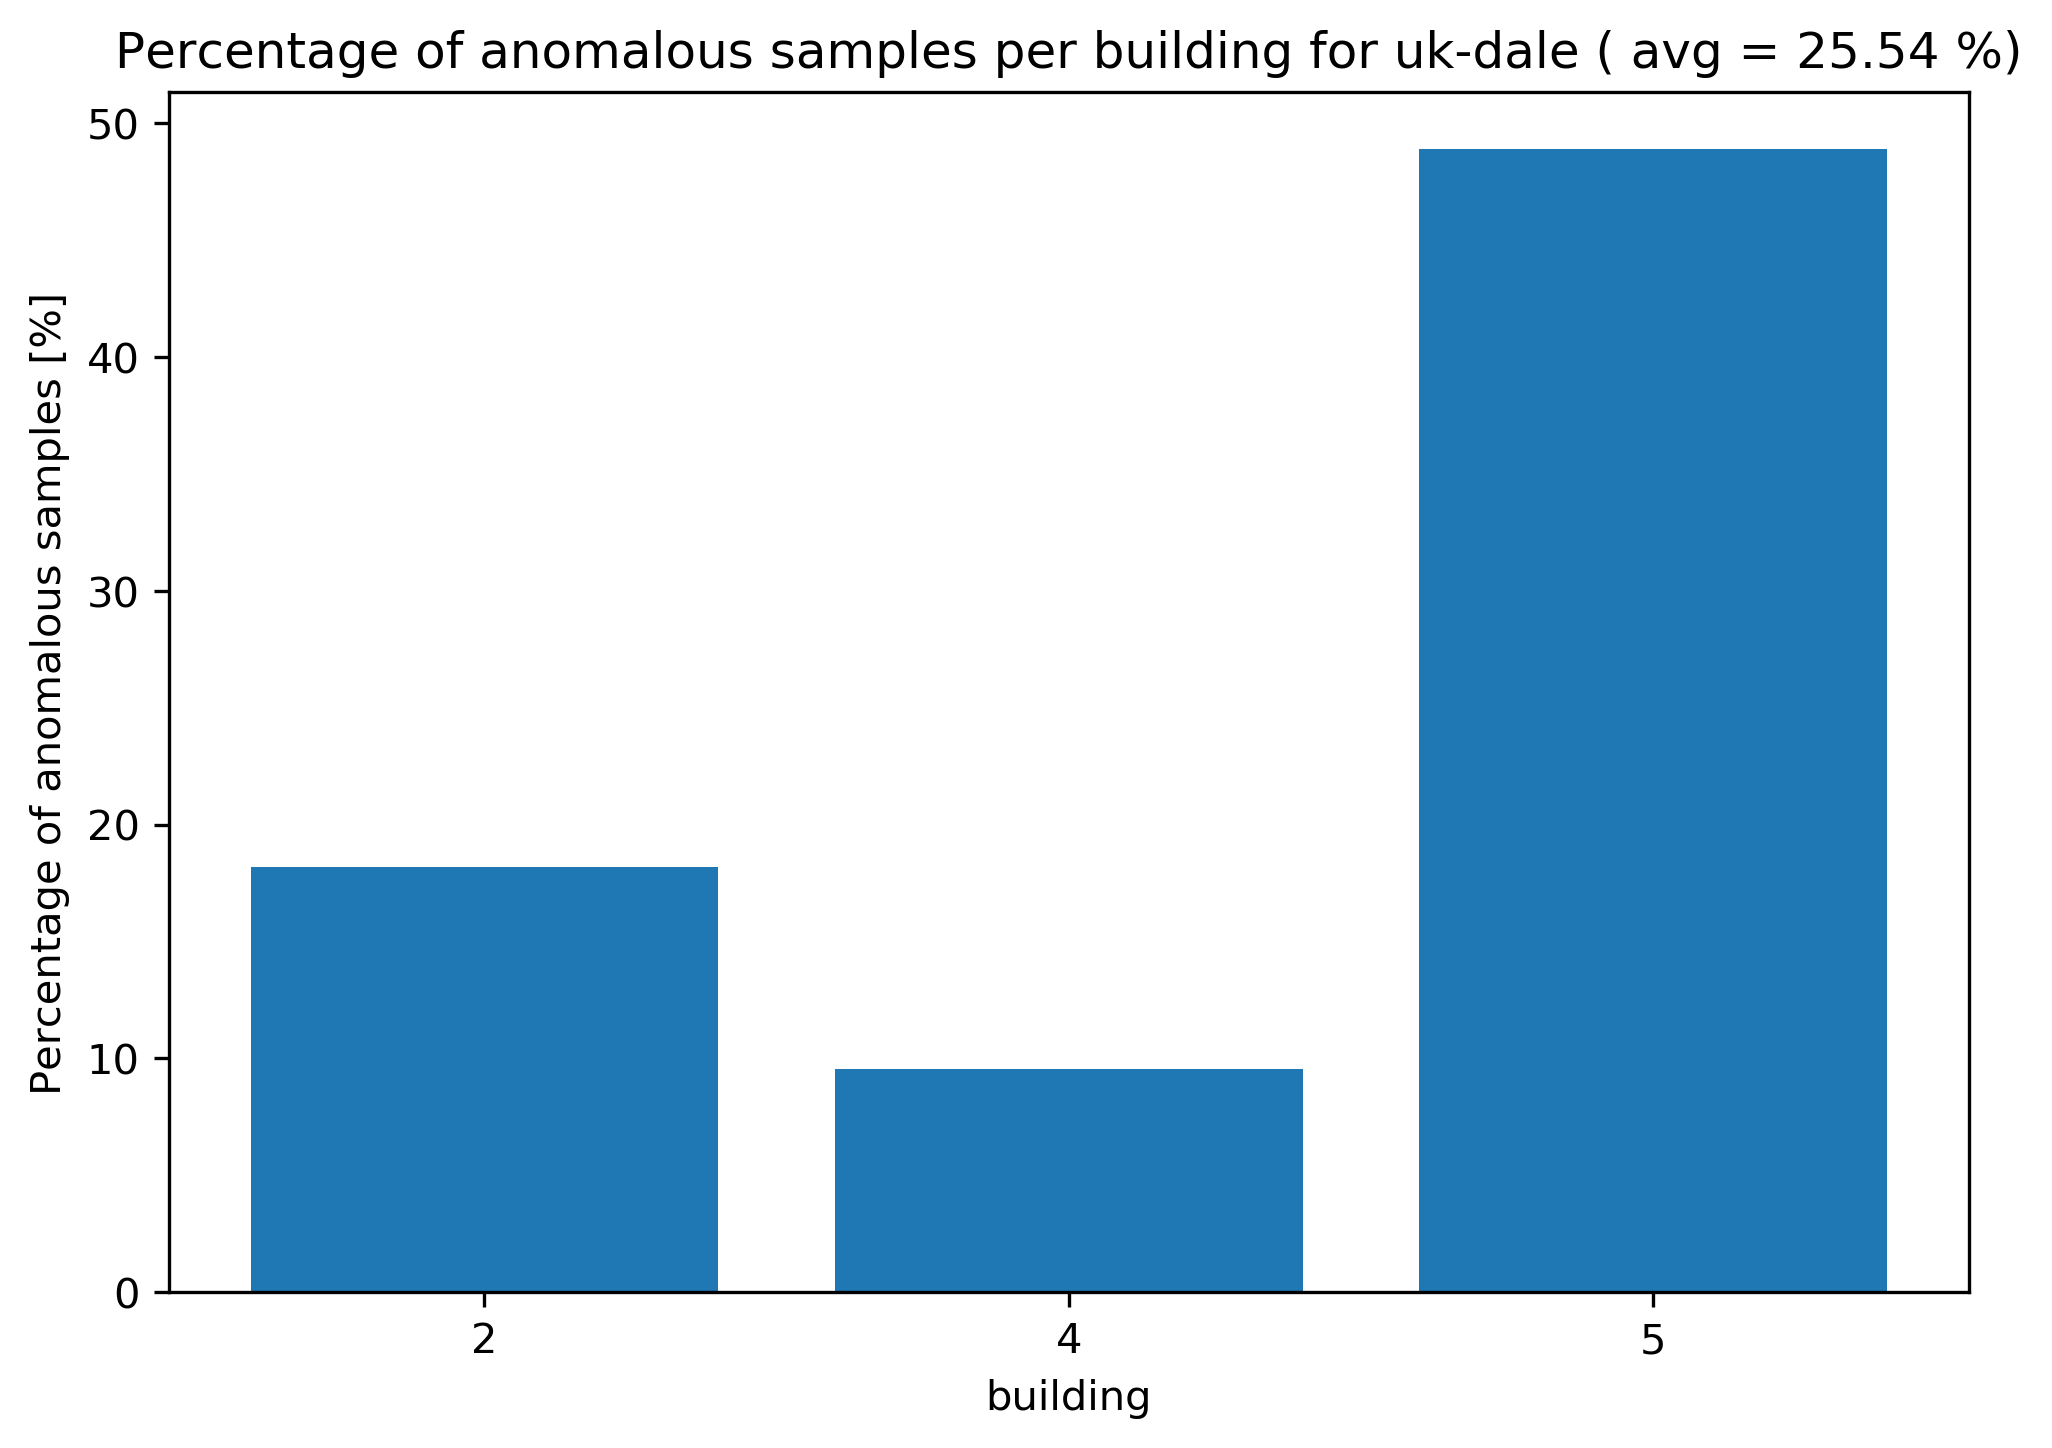
\includegraphics[width=.7\textwidth]{Figures/EC/ukdale_nw_res.png}
	\label{fig:ukdale_res_nw}
\end{figure}

\subsection{ECO}

ECO is of a similar quality as UK-DALE as can be seen in \ref{ssec:ds_eval}, regarding the number of buildings and the length of data.
The results \ref{fig:eco_res}, show that this dataset performed the best, with results of 16.32 \%.

\begin{figure}[H]
	\centering
	\caption{"Results for ECO "}
	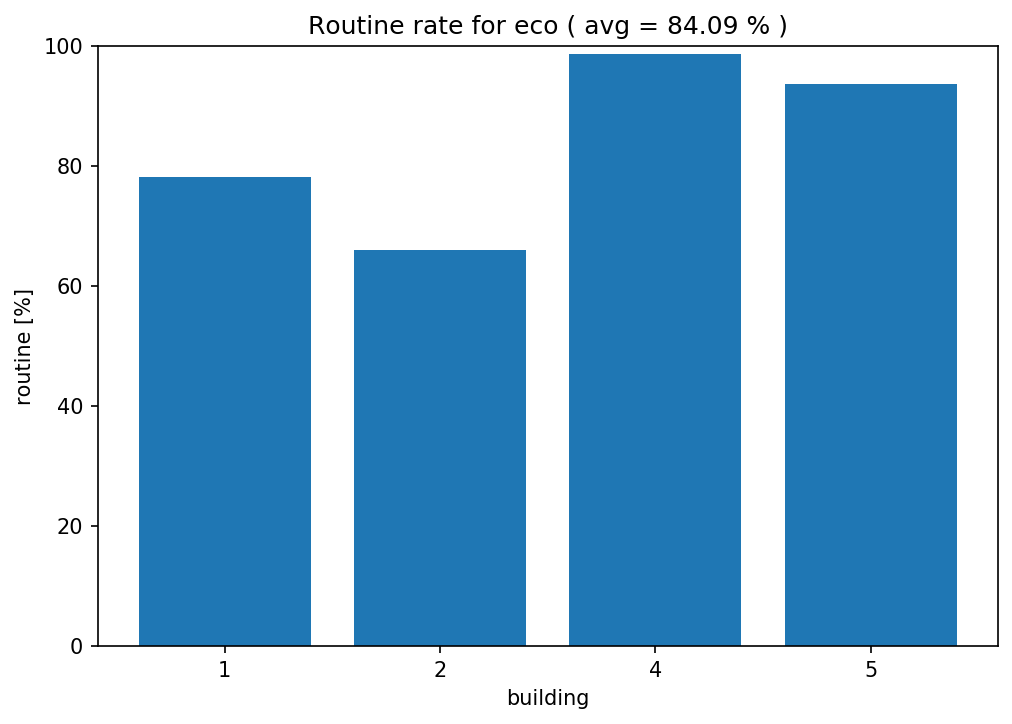
\includegraphics[width=.7\textwidth]{Figures/EC/eco_res_nw_1.png}
	\label{fig:eco_res}
\end{figure}

The same as before we can omit weekend data, which can be seen on \ref{fig:eco_res_nw}. This brings the result down to 15.91 \%. 

\begin{figure}[H]
	\centering
	\caption{"Results for ECO omiting weekends "}
	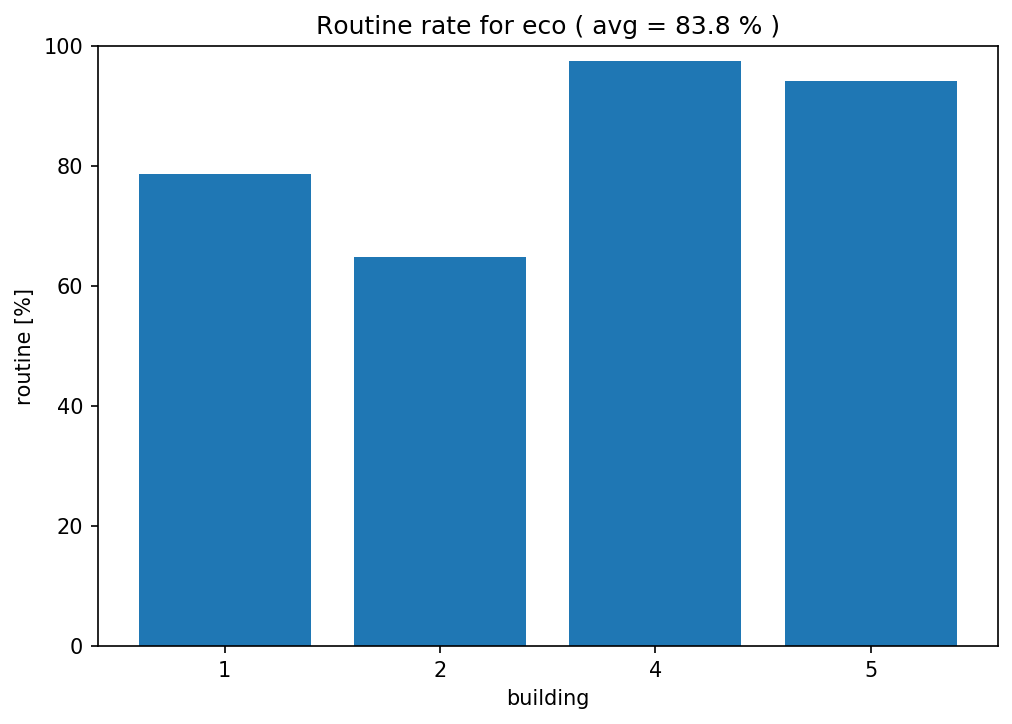
\includegraphics[width=.7\textwidth]{Figures/EC/eco_res.png}
	\label{fig:eco_res_nw}
\end{figure}

\subsection{Combined results}

After combining results from all 24 buildings, the following table \ref{tab:ec_res} can be populated.
The most relevant results can be seen in the last row.
\begin{table}[H]
    \centering
    \caption{Combined percentage of anomolous samples [\%]}
    \begin{tabular}{|l|ll|ll|}
    \hline
    N = 24 &
      \multicolumn{2}{l|}{\begin{tabular}[c]{@{}l@{}}Including \\ weekend data\end{tabular}} &
      \multicolumn{2}{l|}{\begin{tabular}[c]{@{}l@{}}Excluting \\ weekend data\end{tabular}} \\ \hline
    \begin{tabular}[c]{@{}l@{}}Removed \\ min/max\\ outliers\end{tabular} &
      \multicolumn{1}{l|}{train } &
      test &
      \multicolumn{1}{l|}{train} &
      test \\ \hline
    0 & \multicolumn{1}{l|}{15.92} & 23.71 & \multicolumn{1}{l|}{14.39} & 22.78 \\ \hline
    1 & \multicolumn{1}{l|}{16.05} & 23.19 & \multicolumn{1}{l|}{14.45} & 22.11 \\ \hline
    2 & \multicolumn{1}{l|}{16.02} & 22.62 & \multicolumn{1}{l|}{14.43} & 21.64 \\ \hline
    \end{tabular}
    \label{tab:ec_res}
\end{table}

Results show that the algorithm would, on average, label 22 \%of samples as false positive, meaning
every fifth sample could be a false positive. In other words, the algorithm will be 78 \% efficient at 
detecting true anomalies. 


\section{Discussion}

When analyzing these results one important metric is socio-economic status,
such as age, income and number of dwellers in the building. 
Since the datasets did not provide any of this information,
it is hard to make any other conclusions other than the algorithm
works well on an average building.

We know that the reason for installing such a system is that the user is left alone.
We can assume that on average there is more than one dweller in buildings tested.
Since this system would usually be in use by a single dweller,
this would be in favor of our algorithm since it would be 
easier to extract the routine.

One other thing that would be in our favor is that the average person has a lower routine that an elderly person. 
If we take a look at the results, it is possible to see that,
the average home has a low routine during the noon. 
This is because the average person is not at home during noon.
This can be seen on figure \ref{fig:ignored_buckets_22}.
Since the elderly are usually home at that time, this would 
increase the time windows where we can detect the accident.

We could also assume that the older the dweller, the higher the routine. 
The nature of the elderly is that they are more conservative when it comes to changes, and prefer to stick to their routine.
Since the algorithm, works better when usage is periodic, this would also be in our favor. 

Taking all of these assumptions into account, 
there is a possibility that this algorithm would work 
better on the elderly due to their nature.

Since the results on the average building are promising
a test study should be performed. 
This would also prove our assumptions and that this algorithm works 
better on the elderly.


\section{Conclusion}

The question that we tried to answer was:
is this method good enough to be able to efficiently detect anomalies? 
The question that should be asked is,
is the behavior of the users periodic enough, to 
be able to efficiently detect the anomaly?
The answer is: yes, it is.